\section{单纯形法}
\label{sec:opt-lp-simplex}

上一节说明最优解可以在有限个基本可行解中寻找，但不能逐个枚举。单纯形法的想法来自图~\ref{fig:opt-lp-resource-polygon}：站在一个顶点上，检查从它出发的各条边，若某条边能让目标下降，就沿这条边走到下一个顶点；若没有这样的边，就停下。本节把这三步翻译成线性代数：怎样在当前基下判断哪条边下降、走多远、走到哪个新基；随后补上算法还缺的三块——第一个可行基从哪里来，退化时怎样避免原地打转，以及在计算机上怎样稳定、省力地实现这些更新。

\subsection{约化费用与换基更新}
\label{sec:opt-lp-reduced-cost}

\paragraph{用非基变量表示目标}
设$B$是一个可行基，当前基本可行解为$\bm x$。对任意满足$\bm A\bm x=\bm b$的点，把等式拆成基部分与非基部分，$\bm A_B\bm x_B+\bm A_N\bm x_N=\bm b$，于是基变量完全由非基变量决定：
\[
  \bm x_B=\bm A_B^{-1}(\bm b-\bm A_N\bm x_N).
\]
代入目标$\bm c^\top\bm x=\bm c_B^\top\bm x_B+\bm c_N^\top\bm x_N$，得到
\begin{equation}
\label{eq:opt-lp-reduced-cost}
  \bm c^\top\bm x=\bm c_B^\top\bm A_B^{-1}\bm b+\bar{\bm c}_N^\top\bm x_N,
  \qquad
  \bar{\bm c}_N=\bm c_N-\bm A_N^\top\bm A_B^{-\top}\bm c_B.
\end{equation}
第一项是当前顶点的目标值，第二项说明：让非基变量$x_j$从零增加一个单位，目标改变$\bar c_j$。$\bar c_j$称为$x_j$的\term{约化费用}（reduced cost）。记$\bm y=\bm A_B^{-\top}\bm c_B\in\mathbb R^m$，则$\bar c_j=c_j-\bm a_j^\top\bm y$，对基变量同样定义，有$\bar c_j=0$（$j\in B$）。$\bm y$的含义将在第~\ref{sec:opt-lp-duality}节揭晓，这里先把它看作计算约化费用的中间量。

\begin{theorem}[最优性判别]
\label{thm:opt-lp-optimality-criterion}
若可行基$B$的约化费用满足$\bar{\bm c}_N\ge\bm 0$，则它的基本可行解是标准型~\eqref{eq:opt-lp-standard}的全局最优解。
\end{theorem}

\begin{proof}
任取可行点$\bm x'$。它满足$\bm A\bm x'=\bm b$，所以式~\eqref{eq:opt-lp-reduced-cost}对它成立；又$\bm x'_N\ge\bm 0$，故$\bm c^\top\bm x'=\bm c_B^\top\bm A_B^{-1}\bm b+\bar{\bm c}_N^\top\bm x'_N\ge\bm c_B^\top\bm A_B^{-1}\bm b$，右端正是当前基本可行解的目标值。
\end{proof}

判别只比较当前顶点与它相邻的边，结论却是全局的，原因是式~\eqref{eq:opt-lp-reduced-cost}对全部可行点成立，而可行点的非基分量都非负。反过来，若某个$\bar c_j<0$，并不总能断定当前点不是最优：在退化的基下，沿这条边可能一步也走不动（第~\ref{sec:opt-lp-degeneracy}节）。基本可行解非退化时，下面的计算会说明沿这条边确实能使目标严格下降。

\paragraph{沿一条边移动}
选一个$\bar c_j<0$的非基变量$x_j$，称为\term{入基变量}（entering variable）。让$x_j$从$0$增加到$\theta\ge0$，其余非基变量保持为零，基变量随之调整以保持等式成立。由上式，$\bm x_B(\theta)=\bm x_B-\theta\bm A_B^{-1}\bm a_j$。把这一移动写成$\bm x(\theta)=\bm x+\theta\bm d$，方向$\bm d$满足
\begin{equation}
\label{eq:opt-lp-direction}
  d_j=1,\qquad d_k=0\ (k\in N,\ k\ne j),\qquad \bm d_B=-\bm A_B^{-1}\bm a_j.
\end{equation}
直接验证$\bm A\bm d=\bm a_j+\bm A_B\bm d_B=\bm 0$，所以沿$\bm d$移动始终满足等式；目标沿$\bm d$的变化率是$\bm c^\top\bm d=c_j-\bm c_B^\top\bm A_B^{-1}\bm a_j=\bar c_j<0$。在图上，这就是从当前顶点出发、沿一条边离开的方向。

\paragraph{最小比值检验}
沿$\bm d$能走多远，取决于基变量何时降到零。$d_i\ge0$的基变量不会减小；$d_i<0$的基变量在$\theta=x_i/(-d_i)$时降到零。为了保持非负，步长取
\begin{equation}
\label{eq:opt-lp-ratio-test}
  \theta^\star=\min\Bigl\{\frac{x_i}{-d_i}:i\in B,\ d_i<0\Bigr\}.
\end{equation}
这称为\term{最小比值检验}（minimum ratio test）。达到最小值的基变量$x_\ell$首先降到零，称为\term{出基变量}（leaving variable）。若所有$d_i\ge0$，则$\bm x+\theta\bm d$对一切$\theta\ge0$都可行，目标以速率$\bar c_j<0$无限下降，问题无下界，$\bm x$与$\bm d$一起就是这一结论的证据。

\begin{lemma}[换基]
\label{lem:opt-lp-pivot}
设$d_\ell<0$且$\ell$在式~\eqref{eq:opt-lp-ratio-test}中达到最小值。则$B'=(B\setminus\{\ell\})\cup\{j\}$仍是一个基，$\bm x(\theta^\star)$是它的基本可行解，目标值为$\bm c^\top\bm x+\theta^\star\bar c_j$。
\end{lemma}

\begin{proof}
$\bm A_B\bm d_B=-\bm a_j$说明$\bm a_j$用基列表示时，$\bm a_\ell$的系数是$-d_\ell\ne0$。若$B'$的列线性相关，$\bm a_j$就能由$B\setminus\{\ell\}$的列表示，这与表示的唯一性及该系数非零矛盾，所以$\bm A_{B'}$可逆。$\theta^\star$的取法保证$\bm x(\theta^\star)\ge\bm 0$，等式由$\bm A\bm d=\bm 0$保持；它的分量$x_\ell(\theta^\star)=0$，在$N\setminus\{j\}$上的分量也为零，即$B'$以外的分量都为零，所以它就是$B'$的基本可行解。目标值由$\bm c^\top\bm d=\bar c_j$得到。
\end{proof}

用一个新指标替换一个旧指标、从一个基转到相邻的基，称为\term{换基}（pivoting）。几何上，新基本可行解是沿边走到的下一个顶点。$\theta^\star>0$时目标严格下降$\theta^\star|\bar c_j|$；$\theta^\star=0$只可能在当前解退化（某个$x_\ell=0$且$d_\ell<0$）时发生。下面把这些步骤合成算法；初始可行基和出入基的选取规则分别在后两小节给出。

\begin{algorithm}[单纯形法（给定可行基）]
\label{alg:opt-lp-simplex}
\begin{algorithmic}[1]
\Require 满行秩的$\bm A\in\mathbb R^{m\times n}$，$\bm b$，$\bm c$；可行基$B$，即$\bm A_B^{-1}\bm b\ge\bm 0$
\Ensure 最优基本可行解$\bm x$及乘子$\bm y$；或可行点$\bm x$及无下界方向$\bm d$
\Loop
  \State 解$\bm A_B\bm x_B=\bm b$，令$\bm x_N=\bm 0$
  \State 解$\bm A_B^\top\bm y=\bm c_B$，对$j\in N$计算$\bar c_j=c_j-\bm a_j^\top\bm y$
  \If{$\bar c_j\ge0$对全部$j\in N$成立}
    \State \Return 最优解$\bm x$与$\bm y$
  \EndIf
  \State 按入基规则选一个$\bar c_j<0$的$j$
  \State 解$\bm A_B\bm u=\bm a_j$，按式~\eqref{eq:opt-lp-direction}令$\bm d_B=-\bm u$
  \If{$\bm d_B\ge\bm 0$}
    \State \Return 可行点$\bm x$与方向$\bm d$ \Comment{$\bm A\bm d=\bm 0$，$\bm d\ge\bm 0$，$\bm c^\top\bm d<0$}
  \EndIf
  \State 按式~\eqref{eq:opt-lp-ratio-test}求$\theta^\star$，按出基规则选达到最小值的$\ell$
  \State $B\gets(B\setminus\{\ell\})\cup\{j\}$
\EndLoop
\end{algorithmic}
\end{algorithm}

算法每轮的主要工作是两个$m$阶线性方程组和对非基列的定价。入基规则若取约化费用最负的那个，就是最常见的Dantzig规则；它只是一种经验选择，不保证轮数最少。

\paragraph{手算一次}
对资源模型的标准型（例~\ref{ex:opt-lp-resource-standard}），松弛变量提供了现成的可行基$B=\{3,4\}$：$\bm A_B=\bm I$，基本可行解是原点，$x_3=x_4=4$。表~\ref{tab:opt-lp-simplex-run}记录了每一轮的数据。

第$0$轮，$\bm c_B=\bm 0$，所以$\bm y=\bm 0$，约化费用就是$\bar c_1=-3$、$\bar c_2=-2$：两种产品都还没生产，生产任何一种都能增加获利。按Dantzig规则让$x_1$入基。$\bm u=\bm A_B^{-1}\bm a_1=(2,1)^\top$，即$x_1$每增加一单位，$x_3$减少$2$、$x_4$减少$1$；比值为$4/2=2$与$4/1=4$，所以$\theta^\star=2$，$x_3$出基。图~\ref{fig:opt-lp-simplex-path}(b)把这一检验画成了直线：$x_3=4-2\theta$先撞到零，再往前走第一种原料就不够了。新顶点是$(2,0)$，目标值$-6$。

第$1$轮，$B=\{1,4\}$。解$\bm A_B^\top\bm y=\bm c_B$，即$2y_1+y_2=-3$、$y_2=0$，得$\bm y=(-3/2,0)^\top$。于是$\bar c_2=-2-(1\cdot(-3/2)+2\cdot0)=-1/2$，$\bar c_3=0-(-3/2)=3/2$。$x_2$入基；解$\bm A_B\bm u=\bm a_2$，即$2u_1=1$、$u_1+u_4=2$，得$\bm u=(1/2,3/2)^\top$，即$x_2$每增加一单位，$x_1$减少$1/2$、$x_4$减少$3/2$。比值为$2/(1/2)=4$与$2/(3/2)=4/3$，$\theta^\star=4/3$，$x_4$出基。新顶点$(4/3,4/3)$，目标值$-6+(4/3)(-1/2)=-20/3$。

第$2$轮，$B=\{1,2\}$。解$2y_1+y_2=-3$、$y_1+2y_2=-2$，得$\bm y=(-4/3,-1/3)^\top$，$\bar c_3=4/3$、$\bar c_4=1/3$，全部非负。由定理~\ref{thm:opt-lp-optimality-criterion}，$(4/3,4/3)$最优，与图解一致。若第$0$轮改让$x_2$入基，路径会经过另一个顶点$(0,2)$，同样两轮到达最优，见图~\ref{fig:opt-lp-simplex-path}(a)中的虚线。

\begin{table*}[!htbp]
  \centering
  \caption{资源模型上的单纯形法。每轮列出当前基、基本可行解、乘子$\bm y=\bm A_B^{-\top}\bm c_B$、非基变量的约化费用、换基选择与目标值$\bm c^\top\bm x$；最后一轮约化费用全部非负，算法停止。}
  \label{tab:opt-lp-simplex-run}
  \begin{tabular}{@{}cccccccc@{}}
    \toprule
    轮 & $B$ & $\bm x^\top$ & $\bm y^\top$ & 非基约化费用 & 入基 & 比值与出基 & $\bm c^\top\bm x$ \\
    \midrule
    $0$ & $\{3,4\}$ & $(0,0,4,4)$ & $(0,0)$ & $\bar c_1=-3,\ \bar c_2=-2$ & $x_1$ & $x_3{:}\,2,\ x_4{:}\,4$；$x_3$出基 & $0$ \\
    $1$ & $\{1,4\}$ & $(2,0,0,2)$ & $(-\tfrac32,0)$ & $\bar c_2=-\tfrac12,\ \bar c_3=\tfrac32$ & $x_2$ & $x_1{:}\,4,\ x_4{:}\,\tfrac43$；$x_4$出基 & $-6$ \\
    $2$ & $\{1,2\}$ & $(\tfrac43,\tfrac43,0,0)$ & $(-\tfrac43,-\tfrac13)$ & $\bar c_3=\tfrac43,\ \bar c_4=\tfrac13$ & — & 停止 & $-\tfrac{20}3$ \\
    \bottomrule
  \end{tabular}
\end{table*}

\begin{figure}[!htbp]
  \centering
  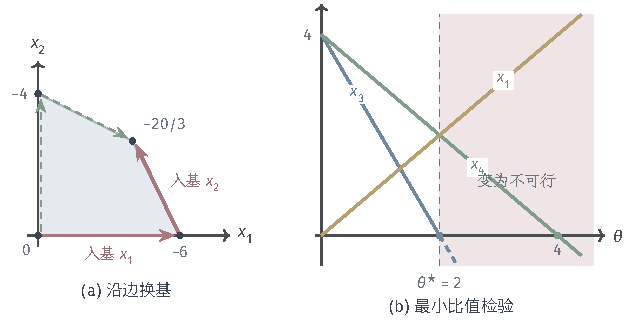
\includegraphics[width=107.262mm]{figures/03-optimization-evolution-and-signals/01-optimization/tikz/c2-simplex-path/figure.pdf}
  \caption{单纯形法沿边换基。(a) 红色实线箭头是表~\ref{tab:opt-lp-simplex-run}中的路径：$x_1$入基走到$(2,0)$，$x_2$入基走到$(4/3,4/3)$；顶点旁的数是标准型目标值$\bm c^\top\bm x$。绿色虚线是先让$x_2$入基的另一条路径。(b) 第$0$轮的最小比值检验：沿边移动步长$\theta$时，基变量$x_3=4-2\theta$与$x_4=4-\theta$线性减小，$x_3$在$\theta^\star=2$处先降到零；浅红区域内$x_3<0$，点已离开可行域。}
  \label{fig:opt-lp-simplex-path}
\end{figure}

\paragraph{与网络单纯形法对照}
图上的最小费用流问题也是标准型线性规划：每条弧$(i,j)$上的流量是一个变量，每个顶点一条守恒约束“净流出等于供需量”，所以弧$(i,j)$对应的列在第$i$行为$1$、第$j$行为$-1$，其余为零。网络单纯形法利用了这一特殊结构，把本节的每一步都换成图上的操作；其树基、节点势和沿环调整的完整推导，可参考\BookChapterRef{chap:graph-optimization}{卷一“图上的组合优化”章}。各行之和为零，所以这些行线性相关；对连通网络删去一行（相当于固定一个根顶点的势为零）后矩阵满行秩，此时基恰好对应生成树。表~\ref{tab:opt-lp-network-simplex}列出了逐项对应。网络单纯形法每一步都只沿树做加减，不需要一般的矩阵分解，这正是特殊结构带来的好处；但这一结构不能代替一般的单纯形法，后者处理的是任意矩阵$\bm A$。卷一的版本还直接处理弧的上界，入弧自身先到达上界时发生“界翻转”；本节只讨论$\bm x\ge\bm 0$的标准型，带上界的变量需要相应推广。

\begin{table}[!htbp]
  \centering
  \caption{一般单纯形法与网络单纯形法的对应。左列是本节的矩阵运算，右列是最小费用流中利用关联矩阵结构实现的同一操作。}
  \label{tab:opt-lp-network-simplex}
  \begin{tabular}{@{}ll@{}}
    \toprule
    一般单纯形法 & 网络单纯形法 \\
    \midrule
    约束行$\bm A\bm x=\bm b$ & 顶点的流量守恒 \\
    列$\bm a_j$ & 弧$(i,j)$，列为$\bm e_i-\bm e_j$ \\
    基$B$ & 生成树的树弧 \\
    乘子$\bm y=\bm A_B^{-\top}\bm c_B$ & 节点势$\bm\pi$（树弧约化费用为零） \\
    约化费用$c_j-\bm a_j^\top\bm y$ & $c_{i,j}-\pi_i+\pi_j$ \\
    方向$\bm d_B=-\bm A_B^{-1}\bm a_j$ & 沿基本环调整流量 \\
    最小比值检验 & 环上剩余量的最小值 \\
    出基变量 & 出弧（阻塞弧） \\
    \bottomrule
  \end{tabular}
\end{table}

\subsection{初始可行基与两阶段法}
\label{sec:opt-lp-two-phase}

算法~\ref{alg:opt-lp-simplex}要求从一个可行基出发。资源模型的约束都是“$\le$”且右端非负，松弛变量的列组成单位矩阵，原点就是基本可行解。这只是幸运的情形。若作坊还承诺两种产品每天合计至少生产$1$件，即$x_1+x_2\ge1$，减去剩余变量$x_5$后写成$x_1+x_2-x_5=1$；这时以$\{3,4,5\}$为基得到$x_5=-1<0$，原点不再可行，也没有现成的单位列可用。一般标准型更是如此，需要专门寻找起点。

\paragraph{第一阶段：构造一个容易起步的辅助问题}
先把$b_i<0$的行整行乘以$-1$，使$\bm b\ge\bm 0$；这不改变可行域。再为每一行引入一个\term{人工变量}（artificial variable）$a_i\ge0$，考虑辅助问题
\begin{equation}
\label{eq:opt-lp-phase-one}
  \min_{\bm x,\bm a}\ \bm 1^\top\bm a
  \quad\text{s.t.}\quad
  \bm A\bm x+\bm a=\bm b,\quad \bm x\ge\bm 0,\quad \bm a\ge\bm 0.
\end{equation}
人工变量的列组成单位矩阵，$(\bm x,\bm a)=(\bm 0,\bm b)$就是它的基本可行解，所以辅助问题有现成的起点；系数矩阵$[\bm A\ \bm I]$也总是满行秩。目标$\bm 1^\top\bm a$不小于零，有下界，配合下一小节的防循环规则，单纯形法会在有限步后停在辅助问题的一个最优基本可行解上。人工变量衡量的是原等式还差多少才能满足，第一阶段就是设法把这些差额压到零。在实际计算中，已有松弛变量可用的行不必再加人工变量，松弛变量的列可以直接充当单位列。

\begin{theorem}[第一阶段的判定]
\label{thm:opt-lp-phase-one}
原问题的可行域$P$非空，当且仅当辅助问题~\eqref{eq:opt-lp-phase-one}的最优值为零。最优值为零时，最优解中的$\bm x$属于$P$。
\end{theorem}

\begin{proof}
若$\bm x\in P$，则$(\bm x,\bm 0)$对辅助问题可行且目标为零，而目标不可能为负，所以最优值为零。反过来，最优值为零时最优解满足$\bm a=\bm 0$，于是$\bm A\bm x=\bm b$、$\bm x\ge\bm 0$。
\end{proof}

第一阶段因此有两种结局。最优值为正时，原问题不可行；第~\ref{sec:opt-lp-certificates}节将说明，此时的终止基还能给出一份可以独立核对的不可行证书。最优值为零时，得到了原问题的一个可行点，但还需要把它整理成原问题的可行基。

\paragraph{把人工变量移出基}
最优值为零时所有人工变量都等于零，但某些人工变量可能仍在基中，只是取值为零。不能直接删去这些列，否则剩下的列数少于行数，基矩阵不再是可逆方阵。设人工变量$a_k$在基中的位置对应$\bm A_B^{-1}$的第$r$行，记该行为$\bm w^\top$。对每个原变量$x_j$，$\bm w^\top\bm a_j$是用当前基表示$\bm a_j$时$a_k$所占的系数。分两种情况：
\begin{itemize}
  \item 若某个非基原变量$x_j$满足$\bm w^\top\bm a_j\ne0$，就让$x_j$入基、$a_k$出基。由引理~\ref{lem:opt-lp-pivot}的证明，新的基矩阵可逆；$a_k=0$，所以这是步长为零的换基，点不动，目标仍为零。
  \item 若全部原变量都满足$\bm w^\top\bm a_j=0$，即$\bm w^\top\bm A=\bm 0^\top$，而$\bm w\ne\bm 0$（它是可逆矩阵的一行），说明$\bm A$的行线性相关。取$w_i\ne0$的某一行$i$，它是其余行的线性组合；原系统可行，所以这一行对应的方程也由其余方程推出，可以删去。
\end{itemize}
重复处理，直到基中没有人工变量。剩下的基全部由原变量组成，是原问题（删去冗余行后）的可行基。随后恢复原目标$\bm c$，从这个基出发运行算法~\ref{alg:opt-lp-simplex}，称为第二阶段。两个阶段合起来就是\term{两阶段法}（two-phase method）。若事先已知$\bm A$满行秩，第二种情况不会出现。

\begin{example}[带最低产量的资源模型]
\label{ex:opt-lp-two-phase}
在资源模型中加入$x_1+x_2-x_5=1$，变量依次为$x_1,\dots,x_5$与人工变量$a$。前两行用松弛变量$x_3,x_4$，第三行用人工变量，初始基为$\{x_3,x_4,a\}$，基本可行解$x_3=x_4=4$、$a=1$。第一阶段目标只对$a$计费用$1$，乘子$\bm y=(0,0,1)^\top$，约化费用$\bar c_1=\bar c_2=-1$、$\bar c_5=1$。让$x_1$入基，$x_1$每增加一单位，$x_3,x_4,a$分别减少$2,1,1$，比值为$2,4,1$，所以$a$出基，步长为$1$。此时$\bm x=(1,0,2,3,0)^\top$，人工变量已经为零，第一阶段最优值为零，基$\{x_1,x_3,x_4\}$是原问题的可行基。

第二阶段恢复$\bm c=(-3,-2,0,0,0)^\top$。在基$\{x_1,x_3,x_4\}$下解得$\bm y=(0,0,-3)^\top$，$\bar c_2=1$、$\bar c_5=-3$，于是$x_5$入基、$x_3$出基，步长$1$，到达$(2,0)$；再让$x_2$入基、$x_4$出基，步长$4/3$，到达$(4/3,4/3)$，此时$x_5=5/3$，约化费用全部非负。整个过程依次经过$(0,0)$、$(1,0)$、$(2,0)$、$(4/3,4/3)$，其中第一个点只对辅助问题可行。
\end{example}

图~\ref{fig:opt-lp-two-phase-flow}汇总了两阶段法的流程。注意它的每一种结局都带有可以核对的数据：可行性由第一阶段判定，最优或无下界由第二阶段判定。

\begin{figure}[!htbp]
  \centering
  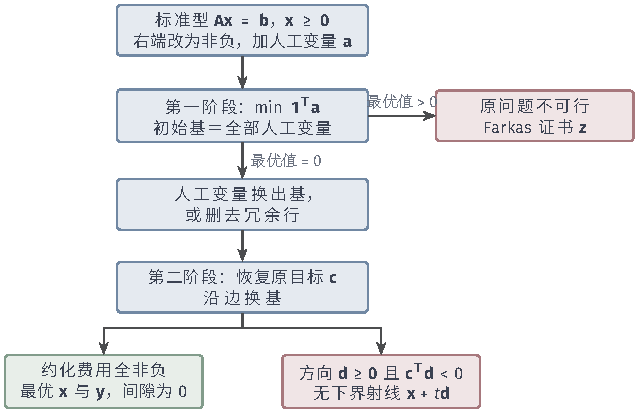
\includegraphics[width=108.112mm]{figures/03-optimization-evolution-and-signals/01-optimization/tikz/c2-two-phase-flow/figure.pdf}
  \caption{两阶段法的流程与三种结局。第一阶段从人工变量组成的单位基出发，最小化人工变量之和：最优值为正时原问题不可行，并得到Farkas证书（第~\ref{sec:opt-lp-certificates}节）；最优值为零时把人工变量换出基或删去冗余行，进入第二阶段。第二阶段以原目标换基，停止时或者得到约化费用全部非负的最优基，或者得到使目标无限下降的可行射线（红框为原问题没有有限最优解的两种情形）。}
  \label{fig:opt-lp-two-phase-flow}
\end{figure}

\subsection{退化、循环与有限终止}
\label{sec:opt-lp-degeneracy}

每次换基目标都不增，基又只有有限个，单纯形法是否一定会停？只有当每一步目标都严格下降时，才能断定不会回到已经访问过的基，从而有限终止。退化恰好破坏这一点。

\paragraph{零步长的换基}
回到第~\ref{sec:opt-lp-bases}小节加了市场限制$x_1\le2$的模型，变量为$x_1,\dots,x_5$，初始基$\{3,4,5\}$。$x_1$入基时，三个比值为$x_3{:}\,4/2=2$、$x_4{:}\,4/1=4$、$x_5{:}\,2/1=2$，$x_3$与$x_5$同时达到最小值。若让$x_5$出基，到达$(2,0)$，基为$\{1,3,4\}$，其中$x_3=0$。

下一轮$\bm y=(0,0,-3)^\top$，$\bar c_2=-2$，$x_2$入基。解$\bm A_B\bm u=\bm a_2$得$x_1,x_3,x_4$随$x_2$增加分别减少$0,1,2$；$x_3$的比值是$0/1=0$，所以$\theta^\star=0$。换基后基变为$\{1,2,4\}$，点仍是$(2,0)$，目标仍是$-6$：这就是一次\term{退化换基}（degenerate pivot）。再下一轮$\bar c_5=-1$，$x_5$入基、$x_4$出基，步长$2/3$，到达$(4/3,4/3)$。图~\ref{fig:opt-lp-degenerate-vertex}画出了这条路径：中间那一步换了基，却没有移动。这里的零步长并非白费，它把$x_2$换进了基，使下一步能沿正确的边离开；但它也说明“目标不增”本身不能保证进展。若在第一步的并列中改让$x_3$出基，则直接得到基$\{1,4,5\}$，下一步一次走到最优点。

\begin{figure}[!htbp]
  \centering
  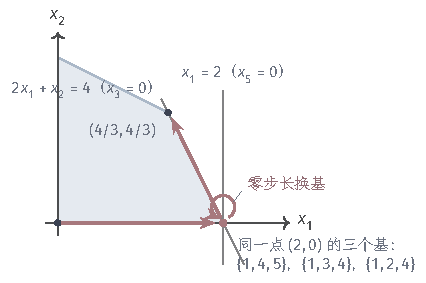
\includegraphics[width=72.164mm]{figures/03-optimization-evolution-and-signals/01-optimization/tikz/c2-degenerate-vertex/figure.pdf}
  \caption{退化顶点与零步长换基。加入$x_1\le2$后可行域不变，但顶点$(2,0)$上有三条边界同时取等号：$x_2=0$、$2x_1+x_2=4$与$x_1=2$。三个不同的基表示这一点。红色路径先从原点走到$(2,0)$，在原地做一次步长为零的换基（小圆弧），再走到最优点$(4/3,4/3)$。}
  \label{fig:opt-lp-degenerate-vertex}
\end{figure}

\paragraph{循环}
若零步长换基接连发生，算法可能在若干个表示同一点的基之间兜圈子，回到已经出现过的基，此后按同样的规则重复同一串换基而永不停止。把“基的序列中某个基重复出现”称为\term{循环}（cycling）。要区分两件事：多个基表示同一点只是退化，本身无害；算法回到同一个基才是循环。已知存在具体的线性规划，在最负约化费用入基、并列时任意选择出基的规则下发生循环\scite{math-bertsimas1997linear}。因此出入基的选择必须写进算法。

\paragraph{Bland规则}
最简单的防循环规则只看变量的编号，它由Bland提出\scite{math-bland1977finite}。

\begin{definition}[Bland规则]
\label{def:opt-lp-bland}
在算法~\ref{alg:opt-lp-simplex}中，入基时在全部$\bar c_j<0$的非基变量中选编号最小的；出基时在式~\eqref{eq:opt-lp-ratio-test}中达到最小比值的全部基变量中选编号最小的。这一选法称为\term{Bland规则}（Bland's rule）。
\end{definition}

\begin{theorem}[Bland规则不会循环]
\label{thm:opt-lp-bland}
设$\bm A$满行秩。按Bland规则执行算法~\ref{alg:opt-lp-simplex}，不会出现循环。
\end{theorem}

\begin{proof}
假设出现循环，基序列$B^{(0)},B^{(1)},\dots,B^{(k)}=B^{(0)}$。目标值沿途不增，又回到原值，所以每次换基的步长都是零，整个循环中基本可行解始终是同一点$\bm x$。称循环中至少有一次入基的变量为“变动变量”；它在某个基中是非基变量，所以$x_j=0$。记变动变量中编号最大的为$t$。

在循环中取一个$x_t$出基的基$B$，设此时入基的是$x_s$；$s$也是变动变量，故$s<t$。沿这次换基的方向$\bm d$（式~\eqref{eq:opt-lp-direction}）有$\bm A\bm d=\bm 0$、$d_s=1$、$\bm c^\top\bm d=\bar c_s<0$；$x_t$出基说明$d_t<0$。再取循环中一个$x_t$入基的基$B'$，记它的乘子为$\bm y'$、约化费用为$\bar{\bm c}'=\bm c-\bm A^\top\bm y'$。Bland规则选中$t$，说明$\bar c'_t<0$，而编号小于$t$的变量都有$\bar c'_j\ge0$；基变量的约化费用为零。

由$\bm A\bm d=\bm 0$，
\[
  \sum_{j=1}^n\bar c'_jd_j=\bm c^\top\bm d-\bm y'^\top\bm A\bm d=\bar c_s<0,
\]
所以存在$r$使$\bar c'_rd_r<0$。$d_r\ne0$说明$r\in B$或$r=s$；$\bar c'_r\ne0$说明$r\notin B'$。$r$在$B$或下一个基中是基变量，在$B'$中是非基变量，所以它是变动变量，$r\le t$。逐一排除：$r=t$时$\bar c'_t<0$且$d_t<0$，乘积为正；$r=s$时$s<t$，$\bar c'_s\ge0$而$d_s=1$，乘积非负。所以$r\in B$、$r<t$，于是$\bar c'_r\ge0$，结合乘积为负得$\bar c'_r>0$、$d_r<0$。但$r$是变动变量，$x_r=0$，在基$B$的比值检验中它的比值是$0/(-d_r)=0=\theta^\star$，与$x_t$并列达到最小值；Bland规则应当选编号更小的$r$出基，而不是$t$。矛盾。
\end{proof}

\begin{theorem}[单纯形法的有限终止]
\label{thm:opt-lp-finite}
设$\bm A$满行秩，从一个可行基出发按Bland规则执行算法~\ref{alg:opt-lp-simplex}（精确算术）。算法在有限轮后停止，要么得到满足$\bar{\bm c}_N\ge\bm 0$的最优基本可行解，要么得到满足$\bm A\bm d=\bm 0$、$\bm d\ge\bm 0$、$\bm c^\top\bm d<0$的方向，说明问题无下界。
\end{theorem}

\begin{proof}
基至多有$\binom nm$个。若算法永不停止，基序列中必有某个基重复出现，形成循环，与定理~\ref{thm:opt-lp-bland}矛盾。算法只在算法~\ref{alg:opt-lp-simplex}的两个返回处停止，两种结论分别由定理~\ref{thm:opt-lp-optimality-criterion}和最小比值检验前的讨论给出。
\end{proof}

两个定理分工明确：有限个基保证序列不能无限地“不重复”，防循环规则保证序列不会“重复”，二者合起来才推出有限终止。同一结论也适用于第一阶段的辅助问题，它的系数矩阵$[\bm A\ \bm I]$满行秩。

\paragraph{代价}
有限终止不等于快。每轮代价由两部分组成：解两个$m$阶线性方程组，以及对至多$n-m$个非基列计算约化费用，后者正比于$\bm A$的非零元个数。总代价还要乘以换基次数，而有限终止的论证只给出“不超过基的个数”这一上界。这个上界不是虚设的：Klee与Minty构造了一族$d$维的变形立方体，在最负约化费用规则下单纯形法要访问全部$2^d$个顶点\scite{math-klee1972simplex}。因此不能从有限终止推出多项式时间保证。在许多实际问题上单纯形法换基次数并不多，但这是经验观察，不是定理。与此对照，第~\ref{chap:constrained-optimization}章介绍的内点法有多项式时间的复杂度保证。此外，以上讨论都假设精确算术；输入数据的位数和舍入误差会影响实际计算，下一小节讨论这一点。

\subsection{单纯形法的数值实现}
\label{sec:opt-lp-revised-simplex}

公式中的$\bm A_B^{-1}$便于推导，却不宜照字面计算。显式求逆每轮要$O(m^3)$次运算，舍入误差也比解方程组更大。

\paragraph{两个线性方程组}
算法~\ref{alg:opt-lp-simplex}只需要逆矩阵与向量的乘积，可以改写为两个方程组：
\[
  \bm A_B^\top\bm y=\bm c_B,\qquad
  \bm A_B\bm u=\bm a_j.
\]
前者给出乘子与约化费用，后者给出方向$\bm d_B=-\bm u$；两者共用同一个基矩阵。保存$\bm A_B$的一个LU分解，两个方程组就都只需前代与回代。只维护基矩阵的分解、而不维护整张表格的实现，称为\term{修正单纯形法}（revised simplex method）\scite{math-nocedal2006numerical}。

\paragraph{更新与重新分解}
相邻两个基只差一列，基矩阵的变化是一个秩一修正，分解可以借助低秩更新而不必重算。但更新会累积舍入误差，大型稀疏问题中还会使分解因子逐渐变稠，所以实现中每隔若干轮（或在误差指标变差时）重新分解一次。$\bm A$通常很稀疏，选择分解的主元次序时要兼顾数值稳定和保持稀疏；定价也不必每轮扫描全部列，可以只检查一部分候选列。这些都改变每轮的实际代价，但不改变算法的数学步骤。

\paragraph{在原模型上检验}
浮点计算得到的$\bm x$不会精确满足等式。设算法报告了基$B$与解$\bm x$，应回到原模型逐项检查：等式残差$\lVert\bm A\bm x-\bm b\rVert$，变量的负部$\max_j\max\{-x_j,0\}$，重新计算的目标值，以及约化费用$\bar c_j$的符号。例如把资源模型的最优解存成七位小数$\bm x=(1.333\,333\,3,\ 1.333\,333\,3,\ 0,\ 0)^\top$，等式残差约为$10^{-7}$，它只是近似可行。容差应当按数据的尺度设置，例如与$\lVert\bm A\rVert$、$\lVert\bm b\rVert$、$\lVert\bm c\rVert$成比例，而不是取一个绝对的小数。

两类情形需要特别留意。约化费用接近零时，它的符号可能由舍入误差决定，算法可能把本应停止的状态当作可以改进，或者反过来；基矩阵接近奇异时，解出的$\bm x_B$和$\bm y$对扰动很敏感，残差小也不代表解准确。因此要分清三件事：算法按规则停止了，结果的残差很小，以及结果已经被证明是原问题的最优解。前两件事都不蕴含第三件。精确算术中，定理~\ref{thm:opt-lp-optimality-criterion}给出了证明；有限精度下，需要一个不依赖算法过程、能直接核对的界，下一节的对偶问题提供的正是这样的界。
